	\documentclass[10pt,oneside]{CBFT_book}
	% Algunos paquetes
	\usepackage{amssymb}
	\usepackage{amsmath}
	\usepackage{graphicx}
	\usepackage{libertine}
	\usepackage[bold-style=TeX]{unicode-math}
	\usepackage{lipsum}

	\usepackage{natbib}
	\setcitestyle{square}

	\usepackage{polyglossia}
	\setdefaultlanguage{spanish}
	



	\usepackage{CBFT.estilo} % Cargo la hoja de estilo

	% Tipografías
	% \setromanfont[Mapping=tex-text]{Linux Libertine O}
	% \setsansfont[Mapping=tex-text]{DejaVu Sans}
	% \setmonofont[Mapping=tex-text]{DejaVu Sans Mono}

	%===================================================================
	%	DOCUMENTO PROPIAMENTE DICHO
	%===================================================================

\begin{document}


% =================================================================================================
\chapter{Simetrías en mecánica cuántica}
% =================================================================================================

En mecánica clásica tenemos el teorema de Noether 
\[
	\dpar{\Lag}{q_i} = 0 \quad \to \quad \dtot{}{t}\left( \dpar{\Lag}{\dot{q}_i} \right) = 
	\dtot{}{t}\left( p_i \right) = 0 \quad \rightarrow \quad \partial p_i = cte.
\]
Y $\Ham, \Lag$ no cambian con la transformación $q_i \longrightarrow q_i + \delta q_i$
\[
	\dpar{\Ham}{q_i} = 0 \quad \to \quad  
	\dtot{}{t}\left( p_i \right) = 0 \quad \rightarrow \quad \partial p_i = cte. 
\]

En mecánica cuántica definiremos un operador unitario $\$$ asociado a traslación/rotación. Pensemos en una 
transformación infinitesimal dada por $\$$
\[
	\mathbb{\$} = \mathbb{1} - i\frac{\varepsilon}{\hbar}G \qquad G \equiv \text{generador hermítico (de 
la transf.)}
\]

Sea el H invariante frente a $\$$, entonces 
\[
	S^\dagger HS = H \quad  \rightarrow \quad [H,\$] = 0 \quad \rightarrow [H,G]=0 \rightarrow
	\dtot{G}{t} = 0 \rightarrow G \;\text{es cte. de movimiento}
\]

Esto significa que el autovalor no varía con el tiempo, Como $[H,G]=0$ se tiene (si no hay degeneración)
\[
	G\Ket{n} = k\Ket{n} \qquad \text{pués} \qquad H(G\Ket{n}) = E_n(k\Ket{n})
\]
invariancia frente a traslaciones $G=\vb{p}$ e invariancia frente a rotaciones $G=\vb{J}$.

\subsection{Simetría de paridad}

Transforma un RHS en LHS. Es decir que hace 
\[
	\vb{x} \longrightarrow - \vb{x}
\]
y solicitaremos un operador unitario llamado paridad que verifique 
\[
	\Ket{\alpha} \longrightarrow \Pi\Ket{\alpha} = \Ket{\alpha'}
\]
si $\Pi$ es unitario y $\Pi^1=\mathbb{1}$ entonces es hermítico.
\begin{figure}[htb]
	\begin{center}
	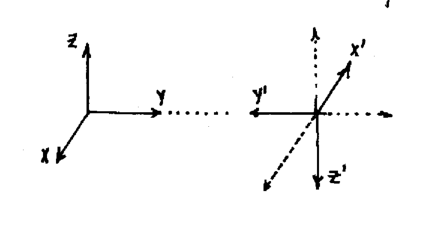
\includegraphics[width=0.6\textwidth]{images/teo2_16.pdf}
	\end{center}
	\caption{}
\end{figure} 
Queremos que refleje el $\Braket{\hat{x}}$ 
\[
	\Braket{\alpha'|\vb{x}|\alpha'} = - \Braket{\alpha|\vb{x}|\alpha} 
\]
\[
	\Braket{\alpha|\Pi^\dagger\vb{x}\Pi|\alpha} = - \Braket{\alpha|\vb{x}|\alpha} \rightarrow
	\Pi^\dagger\vb{x}\Pi = -\vb{x} 
\]
y entonces 
\[
	\{\vb{x},\Pi\} = 0,
\]
anticonmuta con \vb{x}. Debido a ello 
\[
	\Pi\Ket{\vb{x}'} = \Ket{-\vb{x}'} \qquad \Pi^2 \equiv \mathbb{1}
\]
lo cual dice que los autovalores son $\pm 1$ y $\Pi$ es unitario y hermítico.
Como $\hat{\Pi}$ no depende del tiempo 
\[
	\Pi^\dagger\vb{p}\Pi = \Pi^\dagger\dtot{\vb{x}}{t}\Pi = \dtot{}{t}(\Pi^\dagger\vb{p}\Pi) = 
	\dtot{-\vb{x}}{t} \rightarrow \{\vb{p},\Pi\}= 0
\]
y vemos que anticonmuta con \vb{p}.
\vb{x}, \vb{p} son operadores impares. En cambio $\vb{L}=\vb{x}\times\vb{p}$ es un operador par, entonces 
\[
	[\vb{L},\Pi] = 0 \qquad [\vb{J},\Pi] = 0
\]
\begin{figure}[htb]
	\begin{center}
	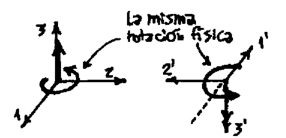
\includegraphics[width=0.6\textwidth]{images/teo2_17.pdf}
	\end{center}
	\caption{}
\end{figure} 
Que conmuta con \vb{J} puede verse de pedirle que 
\[
	[\Pi,\mathcal{D}(R)] = 0 \longrightarrow [\Pi,\vb{J}] = 0 ,
\]
cosa que vale en mecánica clásica, entonces 
\[
	R^{\text{(paridad)}}R^{\text{(rotación)}} = R^{\text{(rotación)}} R^{\text{(paridad)}}
\]
\[
	\Pi^\dagger \Box \Pi =  \begin{cases} +{\Box} \quad \text{par}\quad\text{vector axial( 
	pseudovector)}\\  -\Box \quad \text{impar} \quad \text{vector polar} \end{cases}
\]
\[
	\Pi^\dagger \Box \Pi =  \begin{cases} +\Box \quad \text{par}\quad\text{escalar}\\
	-\Box \quad \text{impar} \quad \text{pseudoescalar} \end{cases}
\]
\[
	\Pi^\dagger \vb{S}\cdot\vb{x} \Pi = \Pi^\dagger \vb{S}\Pi \cdot\Pi^\dagger\vb{x} \Pi =
	\vb{S}\cdot(-\vb{x}) = -\vb{S}\cdot\vb{x}
\]
y $\vb{S}\cdot\vb{x}$ es un pseudoescalar.

\subsection{Función de onda bajo paridad}

\[
	\Psi_\alpha(x') = \Braket{x'|\alpha} = \Braket{x'|\Pi|\alpha} = \Braket{x'|\alpha'} = 
	\Braket{-x'|\alpha}
\]
y entonces la función de onda de un estado al que se le aplicó paridad será 
\[
	\Psi_{\alpha'}(x') = \Psi_\alpha(-x')
\]

Sea $\Ket{\alpha}$ autoestado de paridad, entonces 
\[
	\Pi\Ket{\alpha} = \pm \Ket{\alpha}
\]
los autovalores serán $\pm 1$
\[
	\Braket{x'|\alpha'} = \pm \Braket{x'|\alpha} = \Braket{-x'|\alpha} 
\]
\[
	\Psi_\alpha(-x') = \begin{cases} +\Psi_\alpha(x') \quad \text{función de onda par}\\ 
	-\Psi_\alpha(x') \quad \text{función de onda impar}\\ 
	\end{cases}
\]
no toda función de onda tiene paridad bien definida.

\[
	\vb{x} \to -\vb{x} \longrightarrow \left( r\to r, \theta \to \pi-\theta, \phi \to \phi+\pi \right)
\]
\[
	\Braket{x'|\alpha,\ell,m} = R_\alpha(r) Y_\ell^m(\theta,\phi) \rightarrow \text{con}\vb{x} \; \to 
	-\vb{x} \; \text{será}
\]
\[
	Y_\ell^m(\pi-\theta,\phi+\pi) = (-1)^\ell Y_\ell^m(\theta,\phi)
\]
\[
	\Pi\Ket{\alpha,\ell,m} =  (-1)^\ell \Ket{\alpha,\ell,m}
\]
Como $[\vb{L},\hat{\Pi}]=0$ un autoestado de \vb{L} es autoestado de $\hat{\Pi}$ .

\subsection{Teorema}

Sea $[H,\pi]=0$ y $\Ket{n}$ autoestados no degenerados de $H$ 

	$\Rightarrow$ $\Ket{n}$ es autoestado de $\Pi$.

La demostración 
\[
	\left(\frac{1}{2}\pm \frac{\Pi}{2}\right)\Ket{n} = \frac{\Pi^2\pm\Pi}{2}\Ket{n} = 
	\Pi \left( \frac{\pm 1+\Pi}{2}\right)\Ket{n} = \pm\Pi \frac{1\pm\Pi}{2}\Ket{n}
\]
y entonces es autoestado de paridad con autovalor $\pm 1$. 
\[
	H\frac{1}{2}\left(1\pm\Pi\right)\Ket{n} = \frac{1}{2}E_n\Ket{n} \pm \frac{E_n}{2}\Pi\Ket{n} =
	E_n\left[ \left( \frac{1}{2} \pm \frac{\Pi}{2}\right) \right]
\]
y es autoestado de $H$, de manera que 
\[
	\left( \frac{1\pm\Pi}{2}\right)\Ket{n} = \Ket{n} \Rightarrow \Ket{n} \quad \text{es autoestado de 
paridad}
\]
\[
	\frac{1}{2}\Ket{n} \pm \frac{\Pi}{2}\Ket{n} = \Ket{n}
\]
\[
	\pm \frac{\Pi}{2}\Ket{n} = +\frac{\Ket{n}}{2} \Rightarrow \Pi\Ket{n} = \pm\Ket{n}
\]
Un caso donde falla el teorema 
\[
	[H,\Pi]=0 \quad \text{con} \quad H=\frac{p^2}{2m} 
\]
pero $\Ket{p'}$ no es autoestado de $\Pi$ por la degeneración $\Ket{p'},\Ket{-p'}$ son ambos correspondientes 
al autovalor $p'2/2m$
\[
	\frac{\hat{p}^2}{2m}\Ket{p'} = \frac{{p'}^2}{2m}\Ket{p'} \qquad  \qquad 
	\frac{\hat{p}^2}{2m}\Ket{-p'} = \frac{{p'}^2}{2m}\Ket{-p'}
\]
\[
	\Pi\Ket{p'}= \Ket{-p'}
\]
y $\Ket{p'}$ no es autoestado de $\Pi$.

\subsection{Reglas de selección de paridad $\Pi$}

Sean $\Ket{\alpha}, \Ket{\beta}$ autoestados de paridad 
\[
	\Pi\Ket{\alpha} = \varepsilon_\alpha \Ket{\alpha} \qquad\qquad
	\Pi\Ket{\beta} = \varepsilon_\beta \Ket{\beta}
\]
siendo para el caso impar
\[
	\Braket{\beta|\Box|\alpha} = - \Braket{\beta|\Pi^\dagger\Box\Pi|\alpha} =
	-\varepsilon_\alpha \varepsilon_\beta \Braket{\beta|\Box|\alpha},
\]
y en el caso par
\[
	\Braket{\beta|\Box|\alpha} = \Braket{\beta|\Pi^\dagger\Box\Pi|\alpha} =
	\varepsilon_\alpha \varepsilon_\beta \Braket{\beta|\Box|\alpha}
\]

Si el operador $\Box$ es impar (como $\vb{x}, \vb{p}$) entonces $\varepsilon_\alpha=1,
\varepsilon_\beta=-1$ o bien $\varepsilon_\alpha=-1,\varepsilon_\beta=1$.

Si el operador $\Box$ es par (como $\vb{L}, \vb{S}$) entonces $\varepsilon_\alpha=1,
\varepsilon_\beta=1$ o bien $\varepsilon_\alpha=-1,\varepsilon_\beta=-1$.

\begin{itemize}
 \item Operadores impares solo conectan estados de paridad opuesta
 \item Operadores pares solo conectan estados de la misma paridad 
\end{itemize}

\[
	\Braket{\beta|\vb{x}|\alpha} = 0 
\]
entonces
\[
	\int\int dx'dx''\Braket{\beta|x''}\Braket{x''|\vb{x}|x'}\Braket{x'|\alpha}= 0
\]
y como es $\Braket{x''|\vb{x}|x'} = x' \delta(x' -x'')$
\[
	\int_{-\infty}^{+\infty} dx'\Braket{\beta|x'} x' \Braket{x'|\alpha} =
	\int_{-\infty}^{+\infty} dx'\Psi_\beta^*(x') x' \Psi_\alpha (x')
\]

\section{Inversión temporal (reversión de movimiento)}


En mecánica clásica sería {\it pasar la película hacia atrás}
\[
	t \longrightarrow -t
\]
En sistemas sin fuerzas disipativas se tiene 
\[
	m \ddot{x} = - \dtot{}{x} V(x)
\]
siendo $x(t)$ y $x(-t)$ soluciones de $\vb{F} = m\vb{a}$ pues si $t\to-t$ se tiene
\[
	m \ddot{x} = - \dtot{}{x} V(x)
\]
dado que 
\[
	\dtot[2]{x(t)}{t} = \dtot[2]{x(-t)}{t}
\]

En mecánica cuántica tendremos 
\[
	i \hbar \dpar{\Psi(x,t)}{t} = \left( -\frac{\hbar^2\nabla^2}{2m} + V \right)\Psi(x,t)
\]
y si hacemos el cambio $t\to -t$
\[
	i \hbar \dpar{\Psi(x,-t)}{t} = -i \hbar \dpar{\Psi(x,t)}{t}  = 
	- \left( -\frac{\hbar^2\nabla^2}{2m} + V \right)\Psi(x,t)
\]
se ve que $\Psi(x,-t)$ no es solución de Schrödinger. 

Pero notemos que $\Psi^*(x,-t)$ cumple la ecuación de Schrödinger
\[
	i \hbar \dpar{\Psi^*(x,-t)}{t} = -i \hbar \dpar{\Psi^*(x,t)}{t} 
\]

Entonces necesitamos un operador que respete esta característica.
Necesitaré el producto interno conjugado 
\[
	\Psi_\alpha(x') = \Braket{x'|\alpha} \qquad
	\Psi^*_\alpha(x') = \Braket{x'|\alpha}^* = \Braket{\alpha|x'}
\]
El operador involucrado no será unitario 
\[
	\Ket{\tilde{\alpha}} = \hat{\Theta}\Ket{\alpha} \qquad 
	\Ket{\tilde{\beta}} = \hat{\Theta}\Ket{\beta}
\]
Si $\hat{\Theta}$ unitario se conserva el producto interno 
\[
	\Braket{\hat{\beta}|\hat{\alpha}} = 
	\Braket{\beta|\hat{\Theta}^\dagger\hat{\Theta}|\alpha} =
	\Braket{\beta|\mathbb{1}|\alpha} = \Braket{\beta|\alpha}
\]

Pediremos antiunitariedad y antilinealidad al operador $\hat{\Theta}$
\[
	\Braket{\hat{\beta}|\hat{\alpha}} = \Braket{{\beta}|{\alpha}}^*
\]
\[
	\hat{\Theta}[ C_\alpha\Ket{\alpha} + C_\beta\Ket{\beta}] = 
	C_\alpha^*\hat{\Theta}\Ket{\alpha} + C_\beta^*\hat{\Theta}\Ket{\beta}
\]
siendo lo primero la antiunitariedad y lo segunda la antilinealidad.

Todo operador antiunitario y antilineal puede escribirse como producto 
\[
	\Theta = U K
\]
donde $U$ es unitario y $K$ la conjugación compleja. $K$ no cambia los autoestados, porque en base canónica 
un autoestado tiene un solo elemento (1) que no es nulo.
\[
	K(C\Ket{\alpha}) = CK\Ket{\alpha} = C^*K(\sum_{a'} \Ket{a'}\Braket{a'|\alpha}) =
	C^* (\sum_{a'} \Braket{a'|\alpha}^* K \Ket{a'}) =
	C^* (\sum_{a'} \Braket{a'|\alpha}^* \Ket{a'}) 
\]

Veamos que $UK$ es antiunitario 
\[
	\Ket{\hat{\alpha}} = UK \Ket{\alpha} = \sum_{a'} \Braket{a'|\alpha}^* U\Ket{a'} \qquad \qquad
	\Ket{\hat{\beta}} = UK \Ket{\beta} = \sum_{a''} \Braket{a''|\beta}^* U\Ket{a''}
\]

\[
	\Bra{\hat{\beta}} = \sum_{a''} \Braket{a''|\beta} \Bra{a''}U^\dagger
\]
entonces
\[
	\Braket{\hat{\beta}|\hat{\alpha}} = \sum_{a''} \Braket{a''|\beta} \Bra{a''}U^\dagger
	\sum_{a'} \Braket{a'|\alpha}^* U\Ket{a'}
\]
\[
	\sum_{a',a''} \Braket{a''|\beta} \Braket{a'|\alpha}^* \Bra{a''}U^\dagger U\Ket{a'} =
	\sum_{a'} \Braket{a'|\beta} \Braket{a'|\alpha}^* =  \sum_{a'} \Braket{\beta|a'}^* \Braket{a'|\alpha}^*
	= \Braket{\beta|\alpha}^*
\]
y entonces UK es antinunitario.

Notemos que no se define $\hat{\Theta}^\dagger$ actuando sobre bras. La demostración anterior esperó a 
quitarse de encima $\hat{K}$ para hacer dual conjugado al $\Ket{\tilde{\beta}}$.

\subsection{Operadores ante $\hat{\Theta}$}

Usaremos la notación 
\[
	\Ket{\tilde{\alpha}} = \hat{\Theta} \Ket{\alpha}
\]
donde hay que tener en cuenta 
\[
	\Theta^\dagger \Theta = \mathbb{1}
\]
pues $\Theta^\dagger$ no está definido.

Sería razonable esperar que 
\[
	\Braket{\hat{\alpha}|\vb{p}|\hat{\alpha}} = - \Braket{{\alpha}|\vb{p}|{\alpha}}\qquad 
	\Braket{\hat{\alpha}|\vb{x}|\hat{\alpha}} = \Braket{{\alpha}|\vb{x}|{\alpha}}\qquad 
\]
Sea $\hat{\mathbb{O}}$ un operador hermítico 
\[
	\Braket{\alpha|\mathbb{O}|\alpha} = \Braket{\alpha|\gamma}
\]
\[
	\Braket{\hat{\alpha}|\hat{\gamma}}^* = \Braket{\alpha|\gamma} \Rightarrow 
	\Braket{\hat{\alpha}|\hat{\gamma}} = \Braket{\gamma|\alpha}
\]
y como $\Braket{\hat{\alpha}|\Theta|\gamma} = \Braket{\hat{\alpha}|\Theta\mathbb{O}|\alpha}$.
Luego metemos un $\Theta^{-1}\Theta = 1$
\[
	\Braket{\hat{\alpha}|\Theta\mathbb{O}\Theta^{-1}\Theta|\alpha} =
	\Braket{\hat{\alpha}|\Theta\mathbb{O}\Theta^{-1}|\hat{\alpha}} = \Braket{\alpha|\mathbb{O}|\alpha}
\]

Notamos que no se aplica $\Theta$ sobre bra alguno y tenemos $\Theta$ no unitario. Entonces requeriremos 
\[
	\Theta \hat{p} \Theta^{-1} = -\hat{p} \qquad \Theta \hat{j} \Theta^{-1} = -\hat{j}
\]
\[
	\hat{\Theta}\hat{p} = -\hat{p}\hat{\Theta} \quad \Rightarrow 
	\quad \{ \hat{\Theta},\hat{p}\} = 0
\]
como para $\vb{p},\vb{J}$ operadores impares 
\[
	\Theta \hat{x} \Theta^{-1} = \hat{x}
\]
\[
	\hat{\Theta}\hat{x} = -\hat{x}\hat{\Theta} \quad \Rightarrow 
	\quad [ \hat{\Theta},\hat{x} ] = 0
\]
y $\vb{x}$ operador par.

Los operadores pares conmutan con $\Theta$,
\[
	= =
\]
\begin{figure}[htb]
	\begin{center}
	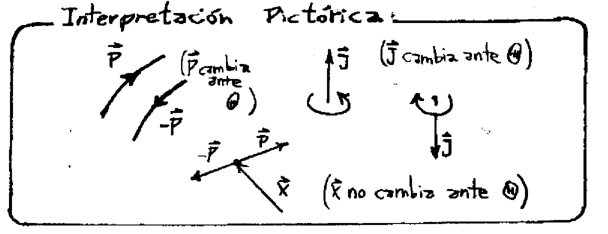
\includegraphics[width=0.6\textwidth]{images/teo2_18.pdf}
	\end{center}
	\caption{}
\end{figure} 
Hamiltoniano ante reversión de movimiento. Veamos la reversión de un sistema en estado $\Ket{\alpha}$
\[
	=
\]
Si el hamiltoniano es invariante ante reversión temporal debería ser lo mismo 
\[
	=
\]
es decir que estamos pidiendo que se obtenga el mismo estado 
\begin{itemize}
 \item Si revertimos el movimiento y evolucionamos $\delta t$.
 \item Si evolucionamos hacia atrás $-\delta t$ y revertimos el movimiento.
\end{itemize}
\begin{figure}[htb]
	\begin{center}
	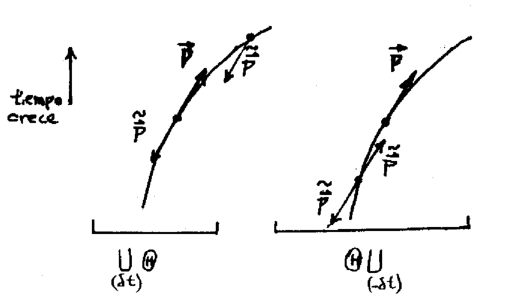
\includegraphics[width=0.6\textwidth]{images/teo2_19.pdf}
	\end{center}
	\caption{}
\end{figure} 
Veamos que vale lo anterior, pensando que si vale se tiene 
\[
	=
\]
\[
	=  \qquad [H,\Theta]=0
\]

Si $\Theta$ era unitario teníamos la relación de anticonmutación $\{ H, \Theta \}=0$ lo cual lleva a absurdos.
\[
	a
\]
Si $\{ H,\Theta \} = 0$
\[
	= \text{H debe ser par frente a $\Theta$}
\]

\subsection{Función de onda}

Sea en $t=0$ un sistema en el estado $\Ket{\alpha}$
\[
	= = 
\]
\[
	\Psi
\]
Esto era lo que {\it vimos} en la ecuación de Schrödinger.

\subsection{Reversión de movimiento sobre \vb{J}}


no tiene sentido porque $J_x,J_y,J_z$ no conmutan entre ellos. Analizaremos $\Ket{\ell,m}$
\[
	\Theta \Ket{\vb{J}} 
\]
\[
	\equiv 
\]

Lo que hace $\Theta$ es invertir la componente de $\hat{z}$ y alterar la fase. Se ve que 
\[
	\Theta^2 = \mathbb{1}
\]

\subsection{Reversión para sistemas de spin $1/2$}

Sea un estado general up de spin $\Ket{\hat{n};+}$, que se obtiene con dos rotaciones 
\[
	Sn
\]
\[
	\Theta
\]
\[
	a
\]
\[
	b
\]
\[
	c
\]

\subsection{Teorema}

Sea $H$ invariante ante $\Theta$ y los $\Ket{n}$ no degenerados, entonces la autofunción de energía puede 
hacerse real tomando una fase apropiada.

Demostración 
\[
	H \Theta  \Ket{n} =
\]
\[
	=
\]
\[
	=
\]

Si le aplico al sistema transformaciones dadas por operadores que conmutan con el H no lo sacamos del 
autoestado en que se encuentra con el paso del tiempo.
En ese sistema solo será razonable medir variables representadas por esos operadores; puesto que de lo 
contrario estamos alterando el sistema y nos es imposible saber donde ha quedado.



% \bibliographystyle{CBFT-apa-good}	% (uses file "apa-good.bst")
% \bibliography{CBFT.Referencias} % La base de datos bibliográfica

\end{document}
